\section{Online {\IterComp} Overview} \label{sec:oic-infra}

    \begin{figure}[t]
        \centering
        \includegraphics[width=\linewidth]{figs/infra-diagram}
        \caption{Overview of the online \itercomp mechanism.}
        \label{fig:infra-diagram}
    \end{figure}

    Although {\itercomp} had been originally proposed as an \textit{offline} optimization strategy, this work shows that this powerful
    technique can be adapted to work in \textit{online} scenarios. Figure~\ref{fig:infra-diagram} shows an overview of how our online
    {\itercomp} mechanism works. On the developers' side, we would traditionally produce an application binary optimized for the inputs
    provided by them. In our approach instead, the program is pre-compiled to LLVM Intermediate Representation (IR) without optimizations
    and is instrumented to measure the amount of work performed and the wall-clock time.
    On the user's side, the online iterative compilation mechanism selects an optimization sequence and compiles the instrumented IR to binary using this sequence.
    Next time the user runs the application, we load and execute the latest binary and measure its work and execution time. We accumulate
    multiple such measurements, executing each input only once, until we can estimate the work efficiency of this optimization sequence
    with high confidence. Finally, we use this information to help us select the next optimization sequence.
    
    In the previous section, we examined the highlighted component of Figure~\ref{fig:infra-diagram}, the \textit{Work Instrumentation}.
    We perform it once and offline, right after the IR is generated before applying optimizations. Its purpose is to measure the amount of
    work performed. The instrumentation creates a global work counter and adds code to a subset of the basic blocks to increment the counter
    each time a block is executed. We calculate the work contribution of each basic block according to the model of Section~\ref{subsec:workmetric}.
    We then select the subset of instrumented basic blocks and the work increments for each one, as discussed in Sections~\ref{subsec:prof}
    and \ref{subsec:relaxed}.
    
    Another component, the \textit{Search Driver}, is responsible for guiding the optimization process. Each selected optimization sequence
    is used for multiple executions of the program in order to gather enough work efficiency measurements. When we are able to
    estimate this work efficiency with a confidence interval narrower than a certain threshold, we can start evaluating a different
    optimization sequence. 

    \subsection{Efficient Optimization Selection and Compilation}

    Most devices have distinct idle and peak usage periods. For example, mobile devices are used intensely during the day and not at all while
    the user is sleeping and the battery is charging~\citep{mpeis16}. Many researchers have identified similar idle and peak usage periods in
    the context of data centers~\citep{armbrust10,chen12b}. The proposed \itercomp infrastructure is very well suited to such scenarios. In
    particular, we can use periods of idleness or underutilization to select the next few optimization sequences to try and to compile the
    corresponding binaries. This approach effectively hides the compilation overhead from the user. During peak periods, we only have to select
    which of the existing binaries to evaluate which introduces almost no overhead.
